\chapter{Methods and Implementation}
\setcounter{chapter}{3}
Summarizing the key points made in chapter \ref{background}, generalization is in large part dependent on the causal robustness of the features that the model learns. The problem of achieving generalization, then, boils down to imposing constraints to the deep learning pipeline such that the model ignores non-causal patterns.

Directly discriminating between causal and non-causal patterns is, however, somewhat intractable. For one, the patterns that neural networks learn are often difficult to identify, and even more difficult to understand intuitively. Though the field of explainable AI has made significant progress in this regard, there simply is not a way to determine the causality of the features learned by DNNs . Moreover, establishing  this causality necessitates a complete understanding of the problem the model is trying to reason about in the first place. If this was at all possible, one might as well use the knowledge required to do so to design a classifier using conventional image-analysis. 

Though establishing what is causal is difficult, establishing what \textit{isn't} causal is not all that complicated. To give a concrete example, consider once again the problem of classifying images of cows and camels. Associating the cow class with grass and the camel class with sand is obviously non-causal, since this pattern would not hold if the model for instance is asked to detect cows on Mars or camels on the Moon. To mitigate this, one may simply collect data of cows and camels in differing backgrounds, but such careful curation of datasets is not typically feasible. A better approach is to instead simply augment the data. In particular, one can generate multiple instances of the same sample but with varied backgrounds. Consistency across this augmented set can then be rewarded in order to bias the model towards learning background-invariant features. 

This, of course, applies to more than just modifying backgrounds: the more of these non-causal changes to the input data-  from this point on referred to as perturbations - are accounted for and modelled, the more spurious correlations are excluded from the search, and the more likely the model is to learn the patterns that are actually causal. After all, a pattern can for all intents and purposes be considered causal when it holds when subjected to all forms of perturbations. 

Thus, though rewarding causal behaviour is intractable, punishing non-causal behaviour is not. All that is required to do so is to be able to apply perturbations that highlight the non-causal reasoning the model employs, quantify the model's sensitivity to these perturbations, then minimize this quantity through optimization. The resulting model will then have learned invariance to whatever causally irrelevant information that the perturbation defines. This property of being invariant to perturbations will be referred to as the consistency of the model. 

Thus, consistency is in effect a surrogate for generalizability; if a model is consistent, it is invariant to non-causal patterns, and if it is invariant to non-causal patterns, it necessarily employs causal patterns. Optimizing for consistency can as a result mitigate both shortcut-learning and underspecification, subject only to the span of the space of perturbations and how well inconsistent behaviour can be quantified. For instance, if the perturbations affect the image such that certain shortcuts are broken, these shortcuts are less likely to be learned. A similar argument can be made for underspecification: if multiple predictors are risk equivalent but nevertheless encode conflicting inductive biases, probing the inductive biases learned by the respective predictors through various perturbations can reveal which are generalizable and which are not.

Naturally, this all presupposes that there is some model that can output all possible perturbations one might desire the model to be invariant to. This is of course not the case. As highlighted by the pervasiveness of adversarial attacks and the relative ineffectiveness of adversarial defences, the perturbations that break DNNs are not necesssarily intuitive and are difficult to analyze in a manner that is conducive to the task of engineering invariance thereto. 

Nevertheless, much stands to be gained if the model learns to be invariant even to a fairly limited space of perturbations. Though generalizability is by no means guaranteed in this case, the odds of learning generalizable features are improved simply because the perturbations limits the types of patterns that a given model can learn. If for instance a white-light endoscopic image is perturbed such that it mimics a narrow-band image, and the model learns to be invariant to this perturbation, predictors that leverage lighting-dependent features will no longer be returned from ERM.

This approach, then, requires two components: a perturbation model, and some form of training procedure that imposes invariance to the transformations that the perturbation model employs - or in other words, learns to be consistent. To this end, a numeric representation of consistency in the context of segmentation needs to be established.
\section{Segmentation Inconsistency Coefficient}
In the context of segmentation, consistency is the ability of the model to output a reasonable segmentation when the input data is subjected to some perturbation. Inconsistency, by the same token, is the extent to which the output changes when subjected to a perturbation beytond what is reasonable. One simple approach to express this numerically would simply be to count the number of pixels that change given some perturbation, and normalize this with respect to the total number of pixels, or in other words calculating the intersection over union, also known as the Jaccard Index, across the perturbed and unperturbed segmentations.  However, the ground truth may of course change as a result of the perturbation - if the image is rotated, for example, the segmentation mask should be rotated accordingly. If an image is globally distorted in some way, the segmentation should exhibit the corresponding distortion. If an image is exposed to low-amplitude additive noise, the segmentation should not really be affected at all, and so on. This, of course, all needs to be taken into account. This can be acheived by discounting the proportion of pixels that is expected to change from the overall metric. Formally, this metric, from this point referred to as the segmentation Inconsistency coefficient (SIC) can be expressed as follows:

Let \(Y:=\{y,\hat{y}:=f(x)\}\) be the set consisting of the segmentation labels (masks) and predictions for the unperturbed samples, where \(f(\cdot)\) denotes the model. Let \(\epsilon(\cdot)\) be some perturbation function. Then, let \(A:=\{a:=\epsilon(y),\hat{a}:=f(\epsilon(x))\}\) be the set consisting of segmentation predictions and masks when the input is subjected to a perturbation. Inconsistency can then be defined by:
\begin{equation}
    L_c = \frac{1}{\sum\{y \cup a \cup \hat{y} \cup \hat{a} \}} \sum \{y\ominus\hat{y}\ominus a\ominus\hat{a}\}
\end{equation}
Where \(\ominus \) denotes the symmetric difference, or in terms of boolean algebra, the XOR operator.
This, as mentioned, corresponds to counting the number of pixels that change after the input is subjected to a perturbation - \(\hat{a}\ominus \hat{y}\), but discounting those we expect to change, \(a\ominus y\). 
It should be noted that this metric is minimised not only if the predictions are both correct and consistent with one another, but also if the predictions are both incorrect, so long as whatever change that occurs is consistent with the expected change. This is illustrated in Figure \ref{loss_fn}
\begin{figure}[h]
    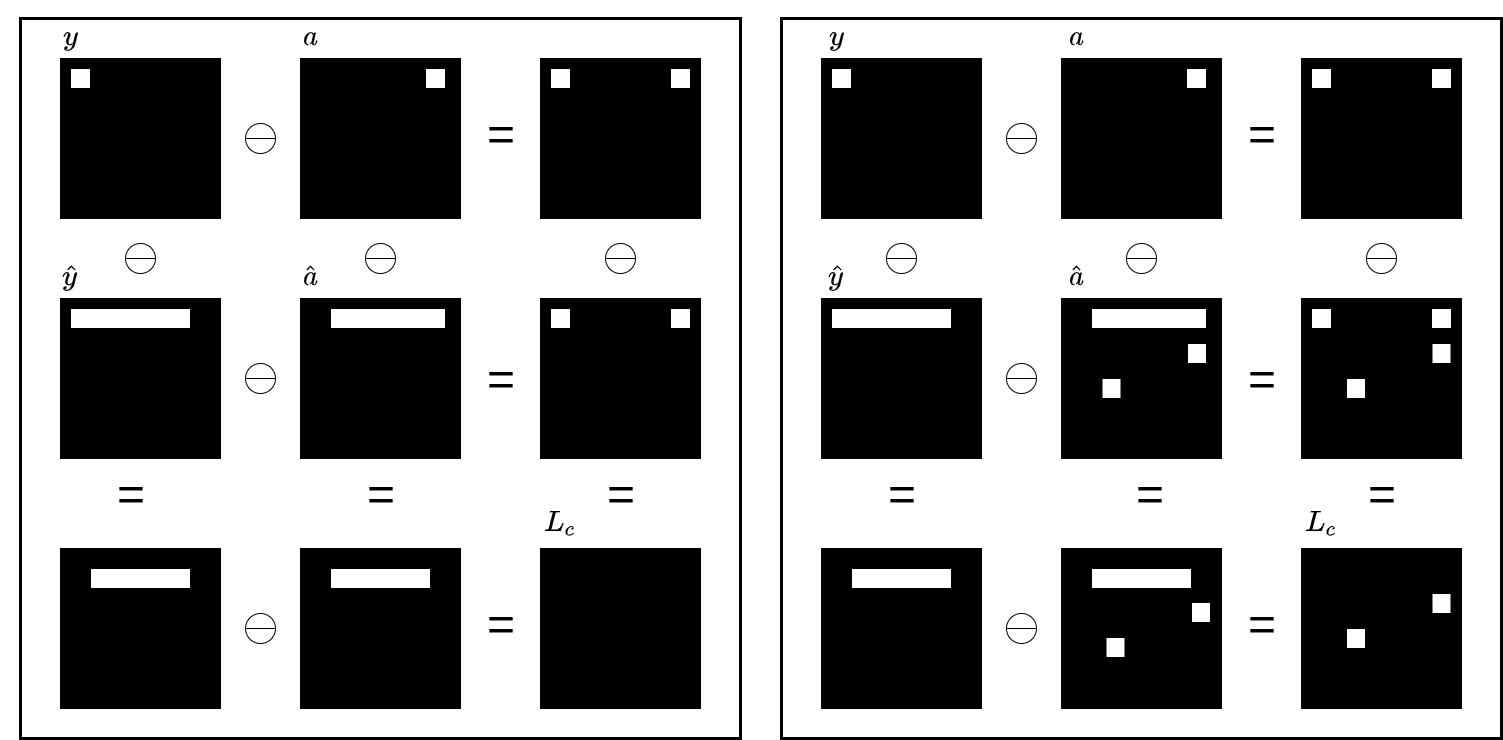
\includegraphics[width=\linewidth]{illustrations/loss_visualisation.drawio.png}
    \caption{Visualisation of SIC sets, where white is a positive prediction. Note that loss is zero regardless of prediction correctness so long as it changes in the expected manner. Note also that the symmetric difference operators are associative. Left shows an instance of consistent but partially incorrect predictions, and right shows an instance of inconsistent but partially correct predictions}
    \label{loss_fn}
\end{figure}  
    
Note, however, that this metric does not presuppose what transformation has occurred. In Figure \ref{loss_fn}, for instance, the change induced by the perturbation may correspond to simply moving the polyp in the image (and replacing the empty space with a believable background), or it may correspond to a rotation by 90 degrees. How this should be analysed with respect to consistency is up to interpretation - one can argue that a rotation should rotate the incorrect predictions as well, or one can argue that it should only rotate the correct component of the prediction. For simplicity, SIC is based on the latter interpretation. 

\section{Consistency Loss}
Similarly to how one can optimize for the Jaccard Index through the Jaccard Loss, so too can one optimize for consistency by using SIC as a component of a loss function. Naturally, using SIC on its own is not really useful since it only expresses consistency, and is wholly agnostic to whatever object it is trying to segment. Consequently, it has to be combined with a some conventional segmentation loss. A simple way to do this would be to simply add them together and normalize, i.e:
\begin{equation*}
    L(Y, A) = \frac{1}{2} \big[L_{seg}(Y)+L_c(Y,A)\big]
\end{equation*}
Preliminary experiments showed that this, however, exhibited some degree of instability. The model would readily get stuck in local minima where its predictions were indeed consistent, but also consistently predicting artifacts. Examples of this can be found in the appendix. To mitigate this, a better loss function is required. Instead of simply adding the respective losses together, one may weight the individual components adaptively according to the segmentation performance. This way, the model will learn generally correct interpretations early in the training, then start weighing consistency more and more as the model sees improvements to its segmentation performance:
    \begin{equation}
        L = (1-IoU)\times L_{seg} + IoU \times L_c
    \end{equation}
        If the Jaccard Index (IoU) is used, this is also equivalent to:
    \begin{equation}
        L = {L_{jac}}^2 + (1-L_{jac})\times L_c
    \end{equation}
Using this formulation, the model will start off trying to learn features that contribute to generally improved segmentation performance, then as segmentation performance improves start principally focusing on learning consistent features. Moreover, if the model starts veering into areas in the loss-landscape that constitute poor segmentation performance, it will self-correct by weighing the segmentation loss more. 

\section{Perturbation Models}
So far, it has been assumed that a perturbation model has been given beforehand. This is of course not the case, and naturally any such model needs to be designed with respect to the domain in question. Rotational invariance makes sense for endoscopic images, for instance, but not for classification of hand-written numbers. Thus, in order to engineer such a model, it is first necessary to establish what invariances are desired for the given task. In the case of polyp-segmentation, it is clear that it is necessary to account for variability in for instance lighting, image-resolution, polyp-size, polyp-shape, polyp-location, camera-quality, color-shifts, blurs, optical distortions, and affine transformations. Thus, a model is required that can (more or less) parametrize this variability. Broadly speaking, these transformations can be categorized as follows:
\begin{itemize}
    \item Pixel-wise variability, which affect only the image, i.e color-shifts, brightness shifts, contrast-shifts,  blurs etc. Practically, this corresponds to changes in lighting conditions, camera motion, dye applications, etc.
    \item Geometric variability, which affect both the image and the segmentation mask by some parametrizable quantity, i.e affine transforms and distortions. Practically, this corresponds to endoscope orientation, optical distortion in the camera, zooming, etc. 
    \item Manifold variablity, which affects both the image and the segmentation mask depending on a learned model of the distribution. Practically, this corresponds to the size, shape and location of the polyps
\end{itemize}
Pixel-wise variability and geometric variability can be modelled fairly trivially through the use of the same transformations typically used in conventional data-augmentation. Manifold-variability, however, is somewhat more difficult, and requires a functional representation of the distribution. \cite{modelbased} and \cite{cyclegan} achieve this through cross-dataset style-transfer, but this of course necessitates multiple datasets. Given only one dataset, a different method must be used. For a classification task, this could for instance be DeepAugment~\cite{deepaugment} or a similar technique. DeepAugment, however, cannot account for the changes in the segmentation mask that should be induced by the augmentations it generates. Consequently, some other generative model wherein the changes in the segmentation mask can be accounted for is required. To this end, a GAN-inpainter can be used. 

\subsubsection{Gan-based polyp inpainting}
As mentioned in Chapter \ref{background}, the use of GANs and other distributional modelling in the context of generalization is typically restricted to image-to-image translation, and typically involve transforming an image drawn from one distribution such that it is iid with a second distribution. This, though interesting and no doubt useful assuming several such datasets are available, has limited practical use. It is not necessarily always the case that there exists multiple datasets depicting identical problems, and merely translating between modalities does not as mentioned earlier in the thesis ensure generalizability.




\subsection{Geometric and pixel-wise transformations}
\section{\alg}
    \subsubsection{Consistency Training}
    \subsubsection{Adversarial Consistency Training}
    \subsubsection{}
\section{Baselines and Generalizability Metrics}
    \subsection{Baseline Models}
        In order to 
    \subsection{Performance Metrics}
    \subsection{Datasets}
\section{Implementation details}
\section{Experiments}
    \subsection{MNV-testing}
    \subsection{Training methods}
